% GNUPLOT: LaTeX picture with Postscript
\begingroup
  \makeatletter
  \providecommand\color[2][]{%
    \GenericError{(gnuplot) \space\space\space\@spaces}{%
      Package color not loaded in conjunction with
      terminal option `colourtext'%
    }{See the gnuplot documentation for explanation.%
    }{Either use 'blacktext' in gnuplot or load the package
      color.sty in LaTeX.}%
    \renewcommand\color[2][]{}%
  }%
  \providecommand\includegraphics[2][]{%
    \GenericError{(gnuplot) \space\space\space\@spaces}{%
      Package graphicx or graphics not loaded%
    }{See the gnuplot documentation for explanation.%
    }{The gnuplot epslatex terminal needs graphicx.sty or graphics.sty.}%
    \renewcommand\includegraphics[2][]{}%
  }%
  \providecommand\rotatebox[2]{#2}%
  \@ifundefined{ifGPcolor}{%
    \newif\ifGPcolor
    \GPcolortrue
  }{}%
  \@ifundefined{ifGPblacktext}{%
    \newif\ifGPblacktext
    \GPblacktexttrue
  }{}%
  % define a \g@addto@macro without @ in the name:
  \let\gplgaddtomacro\g@addto@macro
  % define empty templates for all commands taking text:
  \gdef\gplbacktext{}%
  \gdef\gplfronttext{}%
  \makeatother
  \ifGPblacktext
    % no textcolor at all
    \def\colorrgb#1{}%
    \def\colorgray#1{}%
  \else
    % gray or color?
    \ifGPcolor
      \def\colorrgb#1{\color[rgb]{#1}}%
      \def\colorgray#1{\color[gray]{#1}}%
      \expandafter\def\csname LTw\endcsname{\color{white}}%
      \expandafter\def\csname LTb\endcsname{\color{black}}%
      \expandafter\def\csname LTa\endcsname{\color{black}}%
      \expandafter\def\csname LT0\endcsname{\color[rgb]{1,0,0}}%
      \expandafter\def\csname LT1\endcsname{\color[rgb]{0,1,0}}%
      \expandafter\def\csname LT2\endcsname{\color[rgb]{0,0,1}}%
      \expandafter\def\csname LT3\endcsname{\color[rgb]{1,0,1}}%
      \expandafter\def\csname LT4\endcsname{\color[rgb]{0,1,1}}%
      \expandafter\def\csname LT5\endcsname{\color[rgb]{1,1,0}}%
      \expandafter\def\csname LT6\endcsname{\color[rgb]{0,0,0}}%
      \expandafter\def\csname LT7\endcsname{\color[rgb]{1,0.3,0}}%
      \expandafter\def\csname LT8\endcsname{\color[rgb]{0.5,0.5,0.5}}%
    \else
      % gray
      \def\colorrgb#1{\color{black}}%
      \def\colorgray#1{\color[gray]{#1}}%
      \expandafter\def\csname LTw\endcsname{\color{white}}%
      \expandafter\def\csname LTb\endcsname{\color{black}}%
      \expandafter\def\csname LTa\endcsname{\color{black}}%
      \expandafter\def\csname LT0\endcsname{\color{black}}%
      \expandafter\def\csname LT1\endcsname{\color{black}}%
      \expandafter\def\csname LT2\endcsname{\color{black}}%
      \expandafter\def\csname LT3\endcsname{\color{black}}%
      \expandafter\def\csname LT4\endcsname{\color{black}}%
      \expandafter\def\csname LT5\endcsname{\color{black}}%
      \expandafter\def\csname LT6\endcsname{\color{black}}%
      \expandafter\def\csname LT7\endcsname{\color{black}}%
      \expandafter\def\csname LT8\endcsname{\color{black}}%
    \fi
  \fi
  \setlength{\unitlength}{0.0500bp}%
  \begin{picture}(7632.00,4320.00)%
    \gplgaddtomacro\gplbacktext{%
      \csname LTb\endcsname%
      \put(1008,480){\makebox(0,0)[r]{\strut{} 1}}%
      \csname LTb\endcsname%
      \put(1008,936){\makebox(0,0)[r]{\strut{} 10}}%
      \csname LTb\endcsname%
      \put(1008,1392){\makebox(0,0)[r]{\strut{} 100}}%
      \csname LTb\endcsname%
      \put(1008,1848){\makebox(0,0)[r]{\strut{} 1000}}%
      \csname LTb\endcsname%
      \put(1008,2304){\makebox(0,0)[r]{\strut{} 10000}}%
      \csname LTb\endcsname%
      \put(1008,2760){\makebox(0,0)[r]{\strut{} 100000}}%
      \csname LTb\endcsname%
      \put(1008,3216){\makebox(0,0)[r]{\strut{} 1e+06}}%
      \csname LTb\endcsname%
      \put(1008,3672){\makebox(0,0)[r]{\strut{} 1e+07}}%
      \csname LTb\endcsname%
      \put(1008,4128){\makebox(0,0)[r]{\strut{} 1e+08}}%
      \put(1104,320){\makebox(0,0){\strut{} 0}}%
      \put(1880,320){\makebox(0,0){\strut{} 5}}%
      \put(2656,320){\makebox(0,0){\strut{} 10}}%
      \put(3432,320){\makebox(0,0){\strut{} 15}}%
      \put(4209,320){\makebox(0,0){\strut{} 20}}%
      \put(4985,320){\makebox(0,0){\strut{} 25}}%
      \put(5761,320){\makebox(0,0){\strut{} 30}}%
      \put(160,2304){\rotatebox{90}{\makebox(0,0){\strut{}Runtime (seconds)}}}%
      \put(3432,80){\makebox(0,0){\strut{}Input size (number of measures)}}%
    }%
    \gplgaddtomacro\gplfronttext{%
      \csname LTb\endcsname%
      \put(6897,4008){\makebox(0,0)[r]{\strut{}$n$}}%
      \csname LTb\endcsname%
      \put(6897,3768){\makebox(0,0)[r]{\strut{}$n\log^2(n)$}}%
      \csname LTb\endcsname%
      \put(6897,3528){\makebox(0,0)[r]{\strut{}$2^n$}}%
      \csname LTb\endcsname%
      \put(6897,3288){\makebox(0,0)[r]{\strut{}$2^{2^n}$}}%
      \csname LTb\endcsname%
      \put(6897,3048){\makebox(0,0)[r]{\strut{}original}}%
      \csname LTb\endcsname%
      \put(6897,2808){\makebox(0,0)[r]{\strut{}NR}}%
      \csname LTb\endcsname%
      \put(6897,2568){\makebox(0,0)[r]{\strut{}NRS}}%
      \csname LTb\endcsname%
      \put(6897,2328){\makebox(0,0)[r]{\strut{}NRSU}}%
    }%
    \gplbacktext
    \put(0,0){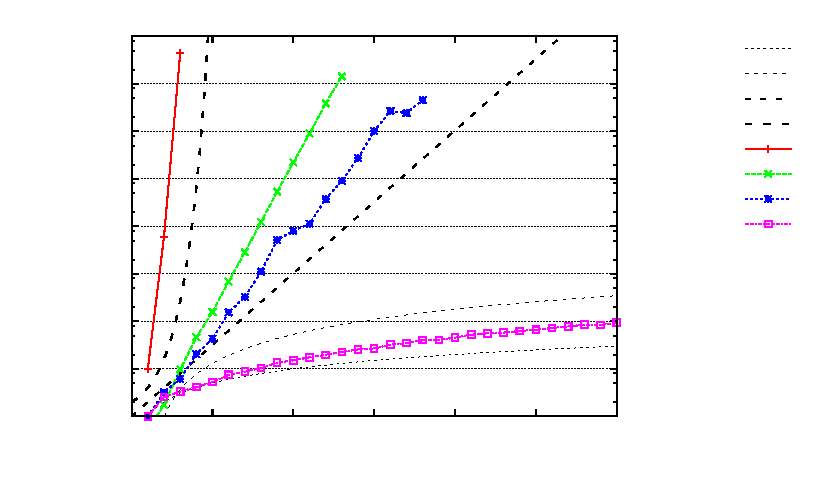
\includegraphics{plot}}%
    \gplfronttext
  \end{picture}%
\endgroup
